\documentclass[aspectratio=169]{beamer}

% packages
\usepackage{graphicx}
  \graphicspath{{figures}}
\usepackage{minted}
\usepackage{amssymb}
\usepackage{tcolorbox}
\usepackage{xcolor}

% strikeout
\usepackage{ulem}

% subfig support
\usepackage{caption}
\usepackage{subcaption}

% packages
\usepackage{biblatex}
  \addbibresource{bibliography.bib}
\usepackage[acronym,nomain]{glossaries}
  \setacronymstyle{long-short}
  \newacronym[shortplural={DoFs},longplural={degrees-of-freedom}]
    {dof}{DoF}{degree-of-freedom}
  \newacronym{fem}{FEM}{the finite element method}
  \newacronym{pde}{PDE}{partial differential equation}
  \newacronym[shortplural={FLOPs},longplural={floating-point operations}]
    {flop}{FLOP}{floating-point operation}
  \newacronym{dag}{DAG}{directed acyclic graph}
  \newacronym{dg}{DG}{discontinous Galerkin}
  \newacronym{poset}{poset}{partially-ordered set}
  \newacronym{rcm}{RCM}{reverse Cuthill-McKee}
  \newacronym{dsl}{DSL}{domain-specific language}
  \newacronym{jit}{JIT}{just-in-time}
  \newacronym{ufl}{UFL}{the Unified Form Language}
  \newacronym{tsfc}{TSFC}{the Two-Stage Form Compiler}
\usepackage{graphicx}
  \graphicspath{{figures}}
\usepackage{todonotes}
\usepackage{hyperref}
\usepackage{subcaption}
\usepackage{amsmath}
% source: https://tex.stackexchange.com/questions/650034/mathbb-font-for-lowercase-letters
\usepackage[bb=libus]{mathalpha}
\usepackage{pgf}
\usepackage{pgfplots}
\usepackage{tikz}
\usepackage{tkz-euclide}
  % \usetikzlibrary{arrows,calc,graphs,graphdrawing,positioning,tikzmark,shapes.geometric,patterns.meta,decorations.pathreplacing,decorations.marking}
  \usetikzlibrary{arrows,calc,graphs,graphdrawing,positioning,tikzmark,shapes.geometric,patterns.meta,decorations.pathreplacing}
  \usegdlibrary{trees}
  \pgfdeclarelayer{background}
  \pgfsetlayers{background,main}
  \tikzstyle{ptlabel} = [anchor=center, color=black, opacity=1]
  \tikzset{font={\small}}
  \tikzset{label style/.append style={font=\small}}
  % source: https://tex.stackexchange.com/questions/356564/macro-for-rounded-polygon-around-some-nodes
  \def\drawpolygon#1,#2;{
    \begin{pgfonlayer}{background}
        \filldraw[line width=28,join=round](#1.center)foreach\A in{#2}{--(\A.center)}--cycle;
        \filldraw[line width=27,join=round,blue!10](#1.center)foreach\A in{#2}{--(\A.center)}--cycle;
    \end{pgfonlayer}
  }

% theme info
\usetheme{firedrake}

% title info
\title{Latest developments in \texttt{pyop3}}
\author{Connor Ward}
\date{13 September 2023}

% macros

% checkbox
% source https://tex.stackexchange.com/questions/16000/creating-boxed-check-mark
\newcommand{\unchecked}{\makebox[0pt][l]{$\square$}\raisebox{.15ex}{\hspace{0.1em}$\quad$}}
\newcommand{\maybe}{\makebox[0pt][l]{$\square$}\raisebox{.15ex}{\hspace{0.1em}$\lozenge$}}
\newcommand{\checked}{\makebox[0pt][l]{$\square$}\raisebox{.15ex}{\hspace{0.1em}$\checkmark$}}

% hacky way to get \pyop2 and \pyop3 as valid macros
% source: https://tex.stackexchange.com/questions/13290/how-to-define-macros-with-numbers-in-them
\def\pyop#1{\ifnum#1=2 {PyOP2}\else \ifnum#1=3 {\texttt{pyop3}}\fi \fi}

\newcommand{\py}{\mintinline{python}}
\newcommand{\clang}{\mintinline{c}}
\newcommand{\closure}{\mathbb{cl}}
\newcommand{\support}{\mathbb{supp}}
\newcommand{\plexstar}{\mathbb{st}}
\newcommand{\cone}{\mathbb{cone}}

\newcommand{\hdiv}{$H(\mathrm{div})$ }
\newcommand{\hcurl}{$H(\mathrm{curl})$ }

\tikzstyle{plexstencil} = [draw=none,fill=blue!30,fill opacity=.4]

\newcommand{\codebgcolor}{black!10}
\newcommand{\mixedstylesetup}{%
  \tikzstyle{v0} = [fill=blue!50];
  \tikzstyle{v1} = [fill=red!65];
}


\newcommand{\myred}[1]{\textcolor{red}{\textbf{#1}}}

% set default parameters for tcolorbox
\tcbset{
  left=2mm
}

% set default minted parameters
\setminted{fontsize=\footnotesize}

% =============================================================================

\begin{document}

\frame{\titlepage}

\begin{frame}{Overview}
  \tableofcontents
\end{frame}

\section{What is \pyop3?}

\begin{frame}{TL;DR}
  \begin{itemize}
    \item A programming language for mathematicians
    \item Comes with a compiler
    \item The language lets you express how to read and write from complicated data structures
  \end{itemize}

  \vfill
\end{frame}

\begin{frame}{In more detail}
  \begin{itemize}
    \item A \myred{domain-specific} programming language for mathematicians \myred{embedded in Python (like UFL)}
    \item Comes with a \myred{just-in-time} compiler \myred{that targets loopy and then C/CUDA/OpenCL}
    \item The language lets you express how to read and write from complicated data structures
    \item \myred{Never need to create a \texttt{PetscSection} ever again!}
  \end{itemize}

  \vfill
\end{frame}

\begin{frame}{Why is this hard?}
  \begin{itemize}
    \item FEM codes have diverse and complicated data structures
    \item These data structures also need to be accessed in non-trivial ways
  \end{itemize}
\end{frame}

\section{A simple-ish example}

\begin{frame}{Outline of a \pyop3 program}
  \begin{enumerate}
    \item Create data structures
    \item Execute loop expressions acting on the data structures
  \end{enumerate}
\end{frame}

\begin{frame}[fragile]{Create a data layout for a 2 cell mesh}
  \noindent
  \begin{minipage}{.4\textwidth}
    \begin{tikzpicture}[scale=.9]
      \tkzDefPoint(0,2){v0}
\tkzDefPoint(2,4){v1}
\tkzDefPoint(2,0){v2}
\tkzDefPoint(4,2){v3}

\tkzDrawSegments(v0,v1 v0,v2 v1,v2 v1,v3 v2,v3)
\tkzDrawPoints(v0,v1,v2,v3)

\tkzDefBarycentricPoint(v0=1.2,v1=1,v2=1) \tkzGetPoint{c0}
\tkzLabelPoint[centered,xshift=-.1cm](c0){3}
\tkzDefBarycentricPoint(v1=1,v2=1,v3=1.2) \tkzGetPoint{c1}
\tkzLabelPoint[centered,xshift=.1cm](c1){7}

\tkzLabelPoint[left](v0){1}
\tkzLabelPoint[above](v1){6}
\tkzLabelPoint[below](v2){4}
\tkzLabelPoint[right](v3){8}

\tkzLabelSegment[below left](v0,v2){0}
\tkzLabelSegment[above left](v0,v1){10}
\tkzLabelSegment[left,xshift=.1cm](v1,v2){5}
\tkzLabelSegment[above right](v1,v3){9}
\tkzLabelSegment[below right](v2,v3){2}

    \end{tikzpicture}
  \end{minipage}%
  \begin{minipage}{.55\textwidth}
    \begin{tcolorbox}
      \begin{minted}[fontsize=\tiny]{python}
mesh_axis = Axis(
  [
    AxisComponent(2, "cells"),
    AxisComponent(5, "edges"),
    AxisComponent(4, "verts"),
  ],
  "mesh"
  permutation=[3, 7, 0, 10, 5, 9, 2, 1, 6, 4, 8],
)
      \end{minted}
    \end{tcolorbox}
  \end{minipage}

  \pause
  \vspace{-2em}

  \begin{center}
    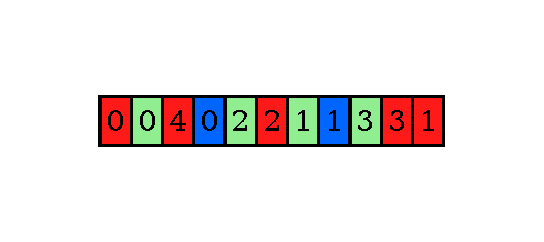
\includegraphics{scripts/two_cell_mesh.gv.pdf}
  \end{center}
\end{frame}

\begin{frame}[fragile]{Now make it a P3 function space}
  \noindent
  \begin{minipage}{.4\textwidth}
    \begin{tikzpicture}[scale=1.5]
      \tkzSetUpStyle[postaction=decorate,decoration={markings,mark=at position .52 with {\arrow[very thick]{stealth}}}]{myarrow}

\newcommand{\defnodes}{
  \tkzDefPoint(0,0){v0}
  \tkzDefShiftPoint[v0](0:2.5){v1}
  \tkzDefShiftPoint[v0](90:2.5){v2}
}

\newcommand{\celldofcolor}{blue!50}
\newcommand{\edgedofcolor}{red!60}
\newcommand{\vertdofcolor}{green!80}

\tikzstyle {cellcolor} = [fill=\celldofcolor];
\tikzstyle {edgecolor} = [fill=\edgedofcolor];
\tikzstyle {vertcolor} = [fill=\vertdofcolor];
\tikzstyle {segment} = [line width=1.2pt];
\tikzstyle {dof} = [draw=black,line width=1.2pt];
\tikzstyle {celldof} = [dof,cellcolor];
\tikzstyle {edgedof} = [dof,edgecolor];
\tikzstyle {vertdof} = [dof,vertcolor];
\tikzstyle {doftext} = [font=\bf];
\tikzstyle {vdof} = [-stealth,draw=red!60,line width=1.9];

\defnodes
\tkzDrawSegment[myarrow,segment](v0,v1)
\tkzDrawSegment[myarrow,segment](v1,v2)
\tkzDrawSegment[myarrow,segment](v0,v2)

\filldraw [vertdof] (v0) node [doftext] {0} circle [radius=7pt];
\filldraw [vertdof] (v1) node [doftext] {1} circle [radius=7pt];
\filldraw [vertdof] (v2) node [doftext] {2} circle [radius=7pt];

% edge dofs
\tkzDefBarycentricPoint(v0=2.3,v1=1) \tkzGetPoint{e0d0}
\filldraw [edgedof] (e0d0) node [doftext] {7} circle [radius=7pt];

\tkzDefBarycentricPoint(v0=1,v1=2.3) \tkzGetPoint{e0d1}
\filldraw [edgedof] (e0d1) node [doftext] {8} circle [radius=7pt];

\tkzDefBarycentricPoint(v1=2.3,v2=1) \tkzGetPoint{e1d0}
\filldraw [edgedof] (e1d0) node [doftext] {3} circle [radius=7pt];

\tkzDefBarycentricPoint(v1=1,v2=2.3) \tkzGetPoint{e1d1}
\filldraw [edgedof] (e1d1) node [doftext] {4} circle [radius=7pt];

\tkzDefBarycentricPoint(v0=2.3,v2=1) \tkzGetPoint{e2d0}
\filldraw [edgedof] (e2d0) node [doftext] {5} circle [radius=7pt];

\tkzDefBarycentricPoint(v0=1,v2=2.3) \tkzGetPoint{e2d1}
\filldraw [edgedof] (e2d1) node [doftext] {6} circle [radius=7pt];

% cell dof
\tkzDefBarycentricPoint(v0=1,v1=1,v2=1) \tkzGetPoint{c0d0}
\filldraw [celldof] (c0d0) node [doftext] {9} circle [radius=7pt];

    \end{tikzpicture}
  \end{minipage}%
  \begin{minipage}{.55\textwidth}
    \begin{tcolorbox}
      \begin{minted}[fontsize=\tiny]{python}
axes = (
  AxisTree(mesh_axis)
    .add_subaxis(Axis(1), mesh_axis.id, "cells")
    .add_subaxis(Axis(2), mesh_axis.id, "edges")
    .add_subaxis(Axis(1), mesh_axis.id, "verts")
)
      \end{minted}
    \end{tcolorbox}
  \end{minipage}

  \pause
  \vspace{-2em}

  \begin{center}
    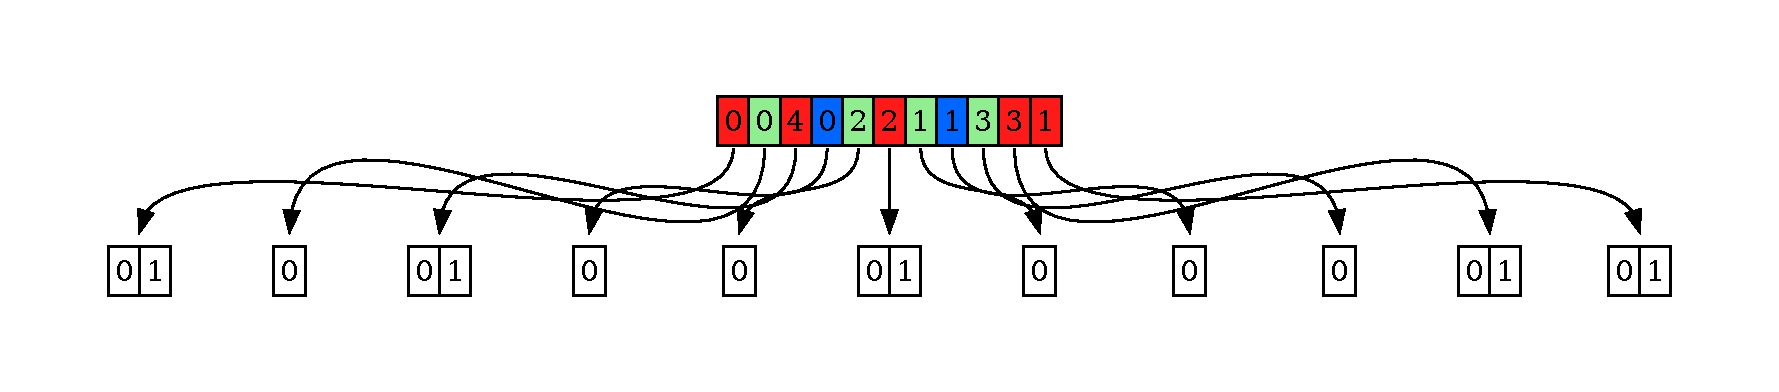
\includegraphics[width=\textwidth]{scripts/two_cell_P3_layout.gv.pdf}
  \end{center}
\end{frame}

\begin{frame}{Now let's do a loop}
  \begin{tikzpicture}
    % define colors
\newcommand{\celldofcolor}{blue!50}
\newcommand{\edgedofcolor}{red!60}
\newcommand{\vertdofcolor}{green!80}

% draw the mesh
\begin{scope}[scale=1.6]
  % styles specific to the mesh
  \tkzSetUpStyle[draw=black,line width=.5]{edge}
  \tkzSetUpStyle[line width=1]{dof}
  \tkzSetUpStyle[dof,draw=\celldofcolor,fill=\celldofcolor]{celldof}
  \tkzSetUpStyle[dof,draw=\edgedofcolor,fill=\edgedofcolor]{edgedof}
  \tkzSetUpStyle[dof,draw=\vertdofcolor,fill=\vertdofcolor]{vertdof}

  % macros
  \newcommand{\defcellmidpoint}[4]{
    \tkzDefBarycentricPoint(#1=1,#2=1,#3=1) \tkzGetPoint{#4}
  }

  \newcommand{\drawcelldof}[3]{
    \defcellmidpoint{#1}{#2}{#3}{#1#2#3}
    \tkzDrawPoint[celldof](#1#2#3)
  }

  \newcommand{\drawedgedof}[2]{
    \tkzDefBarycentricPoint(#1=2,#2=1) \tkzGetPoint{#1#2}
    \tkzDefBarycentricPoint(#1=1,#2=2) \tkzGetPoint{#2#1}
    \tkzDrawPoint[edgedof](#1#2)
    \tkzDrawPoint[edgedof](#2#1)
  }

  \newcommand{\drawvertexdof}[1]{
    \tkzDrawPoint[vertdof](#1)
  }

  % define nodes
  \tkzDefPoints{0/0/v0,0/1/v1,0/2/v2,0/3/v3}
  \tkzDefPoints{1/0/v4,1/1/v5,1/2/v6, 1/3/v7}
  \tkzDefPoints{2/0/v8,2/1/v9,2/2/v10,2/3/v11}
  \tkzDefPoints{3/0/v12,3/1/v13,3/2/v14,3/3/v15}

  % make it look messy
  \tkzDefShiftPoint[v0](0,0){v0}
  \tkzDefShiftPoint[v1](0,.1){v1}
  \tkzDefShiftPoint[v2](-.1,-.1){v2}
  \tkzDefShiftPoint[v3](.2,.1){v3}
  \tkzDefShiftPoint[v4](.1,0){v4}
  \tkzDefShiftPoint[v5](0,0){v5}
  \tkzDefShiftPoint[v6](-.1,0){v6}
  \tkzDefShiftPoint[v7](0,0){v7}
  \tkzDefShiftPoint[v8](0,0){v8}
  \tkzDefShiftPoint[v9](.1,0){v9}
  \tkzDefShiftPoint[v10](0,.1){v10}
  \tkzDefShiftPoint[v11](-.1,.2){v11}
  \tkzDefShiftPoint[v12](0,-.1){v12}
  \tkzDefShiftPoint[v13](.1,-.1){v13}
  \tkzDefShiftPoint[v14](.2,.1){v14}
  \tkzDefShiftPoint[v15](.1,.1){v15}

  % draw the mesh
  \tkzDrawSegments[edge](v0,v1 v1,v2 v2,v3)
  \tkzDrawSegments[edge](v4,v5 v5,v6 v6,v7)
  \tkzDrawSegments[edge](v8,v9 v9,v10 v10,v11)
  \tkzDrawSegments[edge](v12,v13 v13,v14 v14,v15)
  \tkzDrawSegments[edge](v0,v4 v4,v8)
  \tkzDrawSegments[edge](v1,v5 v5,v9)
  \tkzDrawSegments[edge](v2,v6 v6,v10)
  \tkzDrawSegments[edge](v3,v7 v7,v11 v11,v15)
  \tkzDrawSegments[edge](v8,v12 v9,v13 v10,v14)
  \tkzDrawSegments[edge](v1,v4 v1,v6 v3,v6)
  \tkzDrawSegments[edge](v4,v9 v5,v10 v7,v10)
  \tkzDrawSegments[edge](v9,v12 v9,v14 v10,v15)

  % cell DoFs
  \drawcelldof{v0}{v1}{v4}
  \drawcelldof{v1}{v4}{v5}
  \drawcelldof{v1}{v5}{v6}
  \drawcelldof{v1}{v2}{v6}
  \drawcelldof{v2}{v3}{v6}
  \drawcelldof{v3}{v6}{v7}
  \drawcelldof{v4}{v8}{v9}
  \drawcelldof{v4}{v5}{v9}
  \drawcelldof{v5}{v9}{v10}
  \drawcelldof{v5}{v6}{v10}
  \drawcelldof{v6}{v7}{v10}
  \drawcelldof{v7}{v10}{v11}
  \drawcelldof{v8}{v9}{v12}
  \drawcelldof{v9}{v12}{v13}
  \drawcelldof{v9}{v13}{v14}
  \drawcelldof{v9}{v10}{v14}
  \drawcelldof{v10}{v14}{v15}
  \drawcelldof{v10}{v11}{v15}

  % edge DoFs
  \drawedgedof{v0}{v1}
  \drawedgedof{v1}{v2}
  \drawedgedof{v2}{v3}
  \drawedgedof{v4}{v5}
  \drawedgedof{v5}{v6}
  \drawedgedof{v6}{v7}
  \drawedgedof{v8}{v9}
  \drawedgedof{v9}{v10}
  \drawedgedof{v10}{v11}
  \drawedgedof{v12}{v13}
  \drawedgedof{v13}{v14}
  \drawedgedof{v14}{v15}
  \drawedgedof{v0}{v4}
  \drawedgedof{v4}{v8}
  \drawedgedof{v1}{v5}
  \drawedgedof{v5}{v9}
  \drawedgedof{v2}{v6}
  \drawedgedof{v6}{v10}
  \drawedgedof{v3}{v7}
  \drawedgedof{v7}{v11}
  \drawedgedof{v11}{v15}
  \drawedgedof{v8}{v12}
  \drawedgedof{v9}{v13}
  \drawedgedof{v10}{v14}
  \drawedgedof{v1}{v4}
  \drawedgedof{v1}{v6}
  \drawedgedof{v3}{v6}
  \drawedgedof{v4}{v9}
  \drawedgedof{v5}{v10}
  \drawedgedof{v7}{v10}
  \drawedgedof{v9}{v12}
  \drawedgedof{v9}{v14}
  \drawedgedof{v10}{v15}

  % vertex DoFs
  \drawvertexdof{v0}
  \drawvertexdof{v1}
  \drawvertexdof{v2}
  \drawvertexdof{v3}
  \drawvertexdof{v4}
  \drawvertexdof{v5}
  \drawvertexdof{v6}
  \drawvertexdof{v7}
  \drawvertexdof{v8}
  \drawvertexdof{v9}
  \drawvertexdof{v10}
  \drawvertexdof{v11}
  \drawvertexdof{v12}
  \drawvertexdof{v13}
  \drawvertexdof{v14}
  \drawvertexdof{v15}

  % draw a sample patch
  \tkzDefShiftPoint[v5](-.3,-.12){v5patch}
  \tkzDefShiftPoint[v9](.2,-.2){v9patch}
  \tkzDefShiftPoint[v10](.12,.3){v10patch}
  \filldraw[draw=none,fill=black,fill opacity=.15,rounded corners=8]
    (v5patch) -- (v9patch) -- (v10patch) -- cycle;

  % define arrow source
  \tkzDefPoint(1.8,1.65){src1}
\end{scope}

% data layout
\begin{scope}[xshift=7cm,yshift=4.5cm,scale=.5]
  \tkzSetUpStyle[draw=black,line width=.5]{dof}
  \tkzSetUpStyle[dof,fill=\celldofcolor]{celldof}
  \tkzSetUpStyle[dof,fill=\edgedofcolor]{edgedof}
  \tkzSetUpStyle[dof,fill=\vertdofcolor]{vertdof}

  \filldraw[vertdof] (0,0) rectangle ++ (1,1);
  \filldraw[vertdof] (1,0) rectangle ++ (1,1);
  \filldraw[vertdof] (2,0) rectangle ++ (1,1);
  \filldraw[edgedof] (3,0) rectangle ++ (1,1);
  \filldraw[edgedof] (4,0) rectangle ++ (1,1);
  \filldraw[edgedof] (5,0) rectangle ++ (1,1);
  \filldraw[edgedof] (6,0) rectangle ++ (1,1);
  \filldraw[edgedof] (7,0) rectangle ++ (1,1);
  \filldraw[edgedof] (8,0) rectangle ++ (1,1);
  \filldraw[celldof] (9,0) rectangle ++ (1,1);

  % define arrow sources
  \tkzDefPoint(2.7,0){src2}
  \tkzDefPoint(4.5,0){src3}
\end{scope}

% local kernel
\begin{scope}[xshift=11.5cm,yshift=0cm]
  \node [inner sep=0pt,at={(0,1)}]
  {``local kernel"};
  % \node [at={(0,0)}] {"the magic happens"};

  % define arrow source
  \tkzDefPoint(-.5,1.2){src4}
\end{scope}

% connect images
\tkzSetUpStyle[{stealth}-{stealth},shorten >=4pt,shorten <=4pt,line width=1]{connector}
\draw [connector] (src1) to [bend right=25] (src2);
\draw [connector] (src3) to [bend right=25] (src4);

  \end{tikzpicture}
\end{frame}

\begin{frame}[fragile]{Residual assembly in \pyop3}
  \begin{tcolorbox}
    \begin{minted}{text}
for every cell in the mesh:
  collect DoFs found in the cell's closure
  call a local kernel with these DoFs
  scatter the result to a global vector
    \end{minted}
  \end{tcolorbox}

  \pause

  \begin{tcolorbox}
    \begin{minted}{python}
loop(
  c := mesh.cells.index(),
  kernel(func0[closure(c)], ...)
)
    \end{minted}
  \end{tcolorbox}
\end{frame}

\begin{frame}[fragile]{Code generation!}
  \vspace{-1em}

  \begin{tcolorbox}
    \begin{minted}[fontsize=\tiny]{c}
void my_loop(double *func0, int *map0, int *map1, int *layout0, int *layout1, int *layout2, ...) {
  double t_0[10];  // to store the "packed" data

  for (int32_t i_0 = 0; i_0 < 2; ++i_0) {                   // loop over cells
    // pack cell DoFs
    t_0[0] = func0[layout0[i_0]];

    // pack edge DoFs
    for (int32_t i_5 = 0; i_5 < 3; ++i_5) {                 // loop over edges
      for (int32_t i_6 = 0; i_6 < 2; ++i_6) {               // loop over edge DoFs
        j_3 = map0[i_0 * 3 + i_5];                          // select the right edge
        t_0[i_5*2 + i_6 + 1] = func0[layout1[j_3] + i_6];   // pack DoF
      }
    }

    // pack vertex DoFs
    for (int32_t i_7 = 0; i_7 < 3; ++i_7) {                 // loop over vertices
      j_5 = map1[i_0 * 3 + i_7];                            // select the right vertex
      t_0[i_7 + 7] = func0[layout2[j_5]];                   // pack DoF
    }

    // execute the local kernel and unpack the result
    kernel(t_0, ...);
    ...
  }
}
    \end{minted}
  \end{tcolorbox}
\end{frame}

\section{What's the point?}

\begin{frame}{But \pyop2 can already do this, why do we need \pyop3?}
  Is it faster than \pyop2? \\
  \pause
  \myred{No!} \\
  \pause
  Is it as fast as \pyop2? \\
  \pause
  \myred{Not yet!} \\
  \pause
  So why is it useful? \\
  \pause
  \only<6>{\myred{It's not.}}
  \uncover<7->{\sout{\myred{It's not.}}}

  \begin{center}
    \uncover<8->{\myred{Composability!}}
  \end{center}
\end{frame}

\begin{frame}{Why is composability important?}
  \begin{itemize}
    \item Performance optimisation is not the main priority, expressibility is
    \item \pyop2 has limitations:
      \begin{itemize}
        \item Single loop
        \item Single kernel
        \item No map composition
        \item Extruded meshes require invasive code changes
      \end{itemize}
    \item Can do more in fewer lines of code
      \begin{itemize}
        \item \pyop3 compiler is $\sim1000$ lines of code, \pyop2's is $\sim2500$
        \item No special casing for extruded
      \end{itemize}
  \end{itemize}
\end{frame}

\begin{frame}[fragile]{Map composition}
  \begin{itemize}
    \item Interior facet integrals: 
      \begin{tcolorbox}
        \begin{minted}[fontsize=\scriptsize]{python}
loop(facet := mesh.interior_facets, kernel(func0[closure(support(facet))]))
        \end{minted}
      \end{tcolorbox}

    \item Multigrid:
      \begin{tcolorbox}
        \begin{minted}[fontsize=\footnotesize]{python}
closure(fine2coarse(fine_cell))
        \end{minted}
      \end{tcolorbox}
  \end{itemize}
\end{frame}

\begin{frame}[fragile]{Loop and kernel composition: PCPATCH}
  \begin{tcolorbox}
    \begin{minted}{python}
loop(v := mesh.vertices.index, [
  loop(c := star(v).index, [
    kernel1(dat1[closure(c)], "mat"),
    kernel2(dat2[closure(c)], "vec")
  ]),
  solve("mat", "vec", dat3[v])
])
    \end{minted}
  \end{tcolorbox}

  \vspace{-1em}

  \begin{itemize}
    \item We could also try to rewrite SLATE
    \item Loop composition can enable certain tiling optimisations
  \end{itemize}
\end{frame}

\frame{\textbf{And this composability will work with LOADS of data structures...}}

\begin{frame}{Example 1: extruded}
  \noindent
  \begin{minipage}{.2\textwidth}
    \begin{tikzpicture}[scale=.6]
      \tkzDefPoint(0,0){v0v0}
\tkzDefShiftPoint[v0v0](2,0){v1v0}
\tkzDefShiftPoint[v1v0](2,0){v2v0}
\tkzDefShiftPoint[v0v0](0,2){v0v1}
\tkzDefShiftPoint[v1v0](0,2){v1v1}
\tkzDefShiftPoint[v2v0](0,2){v2v1}
\tkzDefShiftPoint[v0v1](0,2){v0v2}
\tkzDefShiftPoint[v1v1](0,2){v1v2}
\tkzDefShiftPoint[v2v1](0,2){v2v2}
\tkzDefShiftPoint[v0v2](0,2){v0v3}
\tkzDefShiftPoint[v1v2](0,2){v1v3}
\tkzDefShiftPoint[v2v2](0,2){v2v3}

% horiz edges
\tkzDrawSegments[red!80,line width=.8](v0v0,v1v0 v1v0,v2v0)
\tkzDrawSegments[line width=.8](v0v1,v1v1 v1v1,v2v1)
\tkzDrawSegments[line width=.8](v0v2,v1v2 v1v2,v2v2)
\tkzDrawSegments[line width=.8](v0v3,v1v3 v1v3,v2v3)

% vert edges
\tkzDrawSegments[line width=.8](v0v0,v0v1 v0v1,v0v2 v0v2,v0v3)
\tkzDrawSegments[line width=.8](v1v0,v1v1 v1v1,v1v2 v1v2,v1v3)
\tkzDrawSegments[line width=.8](v2v0,v2v1 v2v1,v2v2 v2v2,v2v3)

% verts
\tkzDrawPoints[red!80](v0v0,v1v0,v2v0)
\tkzDrawPoints(v0v1,v0v2,v0v3)
\tkzDrawPoints(v1v1,v1v2,v1v3)
\tkzDrawPoints(v2v1,v2v2,v2v3)

% add labels

% lhs
% \tkzDefBarycentricPoint(v0v0=1,v0v1=1) \tkzGetPoint{v0e0}
% \tkzDefBarycentricPoint(v0v1=1,v0v2=1) \tkzGetPoint{v0e1}
% \tkzDefBarycentricPoint(v0v2=1,v0v3=1) \tkzGetPoint{v0e2}
%
% \node [xshift=-1.2cm] (v0v0label) at (v0v0) {$(v_0,v_0)$};
% \node [xshift=-1.2cm] (v0v1label) at (v0v1) {$(v_0,v_1)$};
% \node [xshift=-1.2cm] (v0v2label) at (v0v2) {$(v_0,v_2)$};
% \node [xshift=-1.2cm] (v0v3label) at (v0v3) {$(v_0,v_3)$};
%
% \node [xshift=-1.2cm] (v0e0label) at (v0e0) {$(v_0,e_0)$};
% \node [xshift=-1.2cm] (v0e1label) at (v0e1) {$(v_0,e_1)$};
% \node [xshift=-1.2cm] (v0e2label) at (v0e2) {$(v_0,e_2)$};
%
% \draw [-{stealth},shorten >=2pt] (v0v0label) -- (v0v0);
% \draw [-{stealth},shorten >=2pt] (v0v1label) -- (v0v1);
% \draw [-{stealth},shorten >=2pt] (v0v2label) -- (v0v2);
% \draw [-{stealth},shorten >=2pt] (v0v3label) -- (v0v3);
%
% \draw [-{stealth},shorten >=2pt] (v0e0label) -- (v0e0);
% \draw [-{stealth},shorten >=2pt] (v0e1label) -- (v0e1);
% \draw [-{stealth},shorten >=2pt] (v0e2label) -- (v0e2);
%
% % rhs
% \tkzDefBarycentricPoint(v1v0=1,v2v0=1) \tkzGetPoint{e1e0}
% \tkzDefBarycentricPoint(v1v1=1,v2v1=1) \tkzGetPoint{e1e1}
% \tkzDefBarycentricPoint(v1v2=1,v2v2=1) \tkzGetPoint{e1e2}
%
% \tkzDefBarycentricPoint(v1v0=1,v1v1=1,v2v0=1,v2v1=1) \tkzGetPoint{e1c0}
% \tkzDefBarycentricPoint(v1v1=1,v1v2=1,v2v1=1,v2v2=1) \tkzGetPoint{e1c1}
%
% \node [xshift=1.9cm,yshift=.5cm] (e1e0label) at (e1e0) {$(e_1,e_0)$};
% \node [xshift=1.9cm,yshift=.5cm] (e1e1label) at (e1e1) {$(e_1,e_1)$};
% \node [xshift=1.9cm,yshift=.5cm] (e1e2label) at (e1e2) {$(e_1,e_2)$};
%
% \node [xshift=1.9cm,yshift=.5cm] (e1c0label) at (e1c0) {$(e_1,c_0)$};
% \node [xshift=1.9cm,yshift=.5cm] (e1c1label) at (e1c1) {$(e_1,c_1)$};
%
% \draw [-{stealth},shorten >=2pt] (e1e0label.west) -- (e1e0);
% \draw [-{stealth},shorten >=2pt] (e1e1label.west) -- (e1e1);
% \draw [-{stealth},shorten >=2pt] (e1e2label.west) -- (e1e2);
%
% \draw [-{stealth},shorten >=2pt] (e1c0label.west) -- (e1c0);
% \draw [-{stealth},shorten >=2pt] (e1c1label.west) -- (e1c1);
%
% % bottom labels need to be included in bounding box
% \tkzDefBarycentricPoint(v0v0=1,v1v0=1) \tkzGetPoint{e0}
% \tkzLabelPoint[below](e0){$e_5$}
% \tkzDefBarycentricPoint(v1v0=1,v2v0=1) \tkzGetPoint{e1}
% \tkzLabelPoint[below](e1){$e_1$}
%
% \tkzLabelPoint[below](v0v0){$v_0$}
% \tkzLabelPoint[below](v1v0){$v_3$}
% \tkzLabelPoint[below](v2v0){$v_8$}

    \end{tikzpicture}
  \end{minipage}%
  \begin{minipage}{.8\textwidth}
    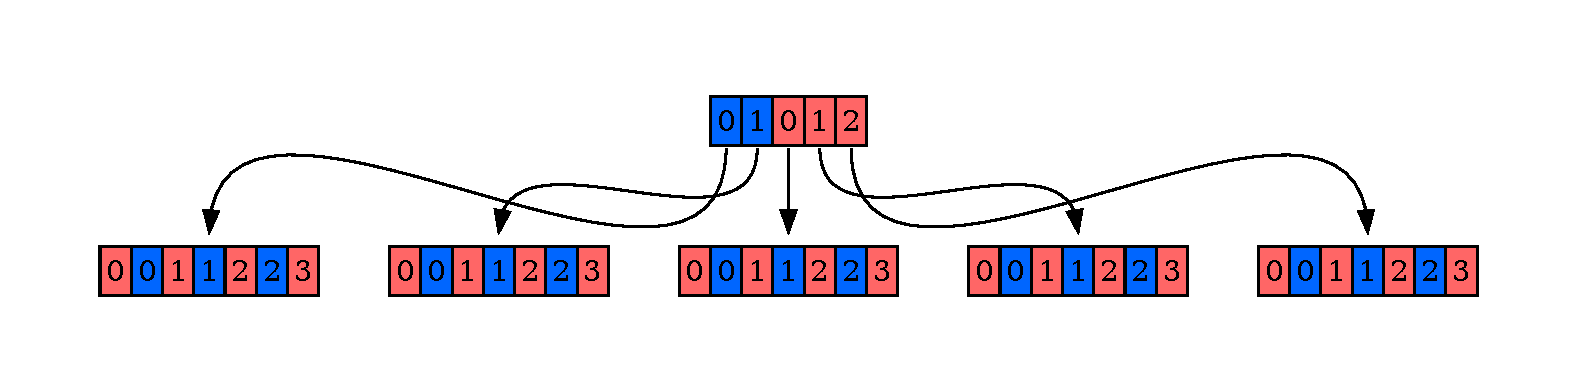
\includegraphics[width=\textwidth]{scripts/extruded_layout.gv.pdf}
  \end{minipage}
\end{frame}

\begin{frame}{Example 2: ragged}
  \begin{center}
    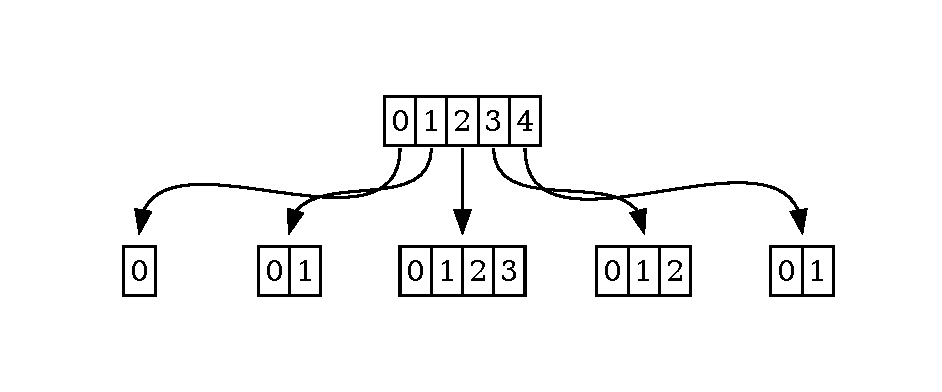
\includegraphics[width=\textwidth]{scripts/ragged_layout.gv.pdf}
  \end{center}

  \vspace{-2em}

  Useful for variable-layer extrusion and PIC.
\end{frame}

\begin{frame}{Example 3: sparse}
  \begin{itemize}
    \item Like ragged (no picture sorry)
    \item Arbitrary sparsity is completely possible
  \end{itemize}
\end{frame}

\begin{frame}{Example 4: ``swapping" axes}
  \begin{figure}
    \centering
    \begin{subfigure}{.65\textwidth}
      \centering
      \begin{tikzpicture}[y=-1cm,scale=.55]
        \mixedstylesetup
        \begin{scope}[xshift=3.25cm, yshift=0cm]
          \filldraw[v0,draw=black] (0,0) rectangle (1,1);
          \filldraw[v1,draw=black] (1,0) rectangle (2,1);
          \node[at={(.5,.5)}, ptlabel] {$V_0$};
          \node[at={(1.5,.5)}, ptlabel] {$V_1$};
        \end{scope}
  
        \begin{scope}[yshift=-2cm]
          \begin{scope}[xshift=0cm]
            \fill[lightgray] (0,0) rectangle (4,1);
            \filldraw[draw=black, fill=white] (0.5,0) rectangle (1.5,1);
            \filldraw[draw=black, fill=white] (1.5,0) rectangle (2.5,1);
            \filldraw[draw=black, fill=white] (2.5,0) rectangle (3.5,1);
            \node[at={(1,.5)}, ptlabel] {$c_0$};
            \node[at={(2,.5)}, ptlabel] {$v_1$};
            \node[at={(3,.5)}, ptlabel] {$c_4$};
            \draw (0,0) -- (4,0);
            \draw (0,1) -- (4,1);
          \end{scope}
  
          \begin{scope}[xshift=4.5cm]
            \fill[lightgray] (0,0) rectangle (4,1);
            \filldraw[draw=black, fill=white] (0.5,0) rectangle (1.5,1);
            \filldraw[draw=black, fill=white] (1.5,0) rectangle (2.5,1);
            \filldraw[draw=black, fill=white] (2.5,0) rectangle (3.5,1);
            \node[at={(1,.5)}, ptlabel] {$c_0$};
            \node[at={(2,.5)}, ptlabel] {$v_1$};
            \node[at={(3,.5)}, ptlabel] {$c_4$};
            \draw (0,0) -- (4,0);
            \draw (0,1) -- (4,1);
          \end{scope}
        \end{scope}
  
        \draw [densely dashed] (3.25,1) -- (0,2);
        \draw [densely dashed] (4.25,1) -- (4,2);
        \draw [densely dashed] (4.25,1) -- ({0+4.5},2);
        \draw [densely dashed] (5.25,1) -- ({4+4.5},2);
  
        \node [at={(9.5,.5)},anchor=center] {Spaces};
        \node [at={(9.5,2.5)},anchor=center] {Points};
      \end{tikzpicture}
    \end{subfigure}
    \hfill
    \begin{subfigure}{.3\textwidth}
      \centering
      \begin{tikzpicture}[x=.8cm,y=-1cm,scale=.7]
        \mixedstylesetup
        \draw (0,0) .. controls (-.2,0) and (-.2,3) .. (0,3);
        \draw (1,0) .. controls (1.2,0) and (1.2,3) .. (1,3);
        \filldraw [v0,rounded corners,draw=none]
          (.1,.05) -- (.9,.05) -- (.9,1.45) -- (.1,1.45) -- cycle;
        \filldraw [v1,rounded corners,draw=none]
          (.1,1.55) -- (.9,1.55) -- (.9,2.95) -- (.1,2.95) -- cycle;
      \end{tikzpicture}
    \end{subfigure}
  
    \vspace{1em}
   
    \begin{subfigure}{.65\textwidth}
      \centering
      \begin{tikzpicture}[y=-1cm,scale=.55]
        \mixedstylesetup
        \begin{scope}[xshift=0cm,yshift=0cm]
          \fill[lightgray] (0,0) rectangle (4,1);
          \filldraw[draw=black, fill=white] (0.5,0) rectangle (1.5,1);
          \filldraw[draw=black, fill=white] (1.5,0) rectangle (2.5,1);
          \filldraw[draw=black, fill=white] (2.5,0) rectangle (3.5,1);
          \node[at={(1,.5)}, ptlabel] {$c_0$};
          \node[at={(2,.5)}, ptlabel] {$v_1$};
          \node[at={(3,.5)}, ptlabel] {$c_4$};
          \draw (0,0) -- (4,0);
          \draw (0,1) -- (4,1);
        \end{scope}
  
        \begin{scope}[xshift=1cm, yshift=-2cm]
          \filldraw[v0,draw=black] (0,0) rectangle (1,1);
          \filldraw[v1,draw=black] (1,0) rectangle (2,1);
          \node[at={(.5,.5)}, ptlabel] {$V_0$};
          \node[at={(1.5,.5)}, ptlabel] {$V_1$};
        \end{scope}
  
        \draw (1.5,1) -- (1,2);
        \draw (2.5,1) -- (3,2);
  
        \node [at={(5,.5)},anchor=center] {Points};
        \node [at={(5,2.5)},anchor=center] {Spaces};
      \end{tikzpicture}
    \end{subfigure}
    \hfill
    \begin{subfigure}{.3\textwidth}
      \centering
      \begin{tikzpicture}[x=.8cm,y=-1cm,scale=.7]
        \mixedstylesetup
        \tikzstyle{entry} = [rounded corners,draw=none];
        \tikzstyle{blue} = [v0,entry];
        \tikzstyle{red} = [v1,entry];
        \draw (0,0) .. controls (-.2,0) and (-.2,3) .. (0,3);
        \draw (1,0) .. controls (1.2,0) and (1.2,3) .. (1,3);
        \filldraw [blue] (.1,.05) -- (.9,.05) -- (.9,.45) -- (.1,.45) -- cycle;
        \filldraw [red] (.1,.55) -- (.9,.55) -- (.9,.95) -- (.1,.95) -- cycle;
        \filldraw [blue] (.1,1.05) -- (.9,1.05) -- (.9,1.45) -- (.1,1.45) -- cycle;
        \filldraw [red] (.1,1.55) -- (.9,1.55) -- (.9,1.95) -- (.1,1.95) -- cycle;
        % \filldraw [blue] (.1,2.05) -- (.9,2.05) -- (.9,2.45) -- (.1,2.45) -- cycle;
        % \filldraw [red] (.1,2.55) -- (.9,2.55) -- (.9,2.95) -- (.1,2.95) -- cycle;
        % ellipsis
        \filldraw [fill=black] (.5,2.2) circle (.5pt);
        \filldraw [fill=black] (.5,2.5) circle (.5pt);
        \filldraw [fill=black] (.5,2.8) circle (.5pt);
      \end{tikzpicture}
      \label{fig:mixedreorder_inner_vec}
    \end{subfigure}
  \end{figure}
\end{frame}

\begin{frame}{Summary}
  \begin{itemize}
    \item \pyop3 is a DSL/compiler framework for writing kernels with non-trivial access patterns
    \item It can do everything \pyop2 can do, and more!
    \item WIP
  \end{itemize}
\end{frame}

\end{document}
